\chapter{Introduction} % Main chapter title
%\selectlanguage{serbianc}
%\sffamily
%\fontencoding{OT2}\fontfamily{Tempora-TLF}\selectfont

Many real systems, such as brain network, social organizations, cities or even biological systems, can be represented as a complex systems. The common property of these systems is that they are composed of many interacting elements. Still, to describe the properties of the system, we can not conclude too much from the behaviour of a single individual. Due to specific interactions, without any central force, in the complex system emergence, the collective behaviour \cite{kwapien2012}. The structure of the brain network and its properties are fundamental for brain functioning, while an emergent phenomenon is human intelligence. In societies, people's interactions lead to civilization, economy, formation of social groups. Also, the animal populations show different levels of organization: such as bird flocks or schools of fishes \cite{thurner2018}.

An important property of the complex systems is called universality \cite{binney1992}. %The empirical analysis showed that universality is characteristic of many collective social phenomena  \cite{chatterjee2013, radicchi2008}. 
Even the growth of social groups, such as cities, follow universal patterns. The probability distribution of the city sizes in one country follows the same laws, with a similar exponent for all countries \cite{barthelemy2019, fazio2015pareto}. However, the distribution of company sizes follows log-normal behavior and remains stable over decades \cite{amaral1997scaling, stanley1996scaling}. Understanding how universalities in the system emerge is the focus of statistical physics of complex systems \cite{verbavatz2020}. The time between two messages is described with power-law distribution. The exponent is universal across different media \cite{garas2012emotional}. The other examples of universality include the votes in elections \cite{fortunato2007scaling, chatterjee2013} and citations of scientific publications \cite{radicchi2008}.

%Emergent collective behavior is an indispensable property of complex systems \cite{ladyman2013}. It occurs as a consequence of interactions between a large number of units that compose a complex system, and it cannot be easily predicted from the knowledge about the behavior of these units. The previous research offers a definite proof that the structure of the interaction network is inextricably associated with dynamic and function of the complex system \cite{barrat2008, pascual2006, castellano2009, gosak2018, arenas2008, boccaletti2016, chen2018, kuga2018}. The structure of complex networks is essential for understanding the evolution and function of various complex systems \cite{boccaletti2006,newman2010, holme2012, boccaletti2014}. 

The research in complex systems focuses on the interactions between its units. The interactions are not homogeneous; as the system evolves, we also find that interactions become specific and nonlinear \cite{thurner2018}. Knowing how units of the system are connected, we can determine the emergence of the collective behaviour of the system \cite{ladyman2013}. For the brain network, we can construct representation with neurons and synapses, representing the brain connectivity. Neurons in the same brain area are closely connected \cite{latora2017complex}.
Similarly, we can define communication between people. The structure of these interactions gives us insights, for example, how information propagates through the system. The presence of people with many connections can lead to faster information flow. 

Despite the differences between complex systems, they can be studied using the same techniques. The natural extension of the complex system is the network, sets of nodes (vertices) and links (edges). Elements in the system are nodes, while interactions between them are given as edges. This approximation allows us to treat equally social \cite{myers2014, sarigol2014} (graph of actors) , biological (network of proteins) \cite{fraiman2009ising, schneider2011modeling} or even technological systems (internet, traffic) \cite{costa2007characterization, costa2011analyzing, newman2003structure}. The complex network theory has applications in different fields, and the availability of big data and great computational efforts incurs its development. 

The complex network theory originates from the graph theory in mathematics. 
The first mathematical problem solved using graph theory was $Konigsberg$ problem of seven bridges. The city $Konigsberg$ had seven bridges connecting the city's parts across the river and the island in the middle. The question was, is it possible to find a walk that crosses all seven bridges only once. Representing the problem as a graph, Euler managed to simplify the problem; the parts of the land are represented as nodes while bridges between them are links. Crossing each bridge only once is possible if each part of the land has an even number of connections. It makes possible to enter one part of the land from one bridge and leave it on the other. As each node has an odd number of connections, in this case, it is not possible; %see Fig. \ref{fig:Krgraph}.

%\begin{figure}[!ht]
%	\centering
%	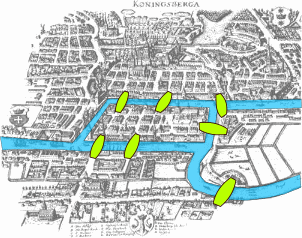
\includegraphics[width=0.3\linewidth]{Konigsberg_bridges.png} \hspace{2cm}
%	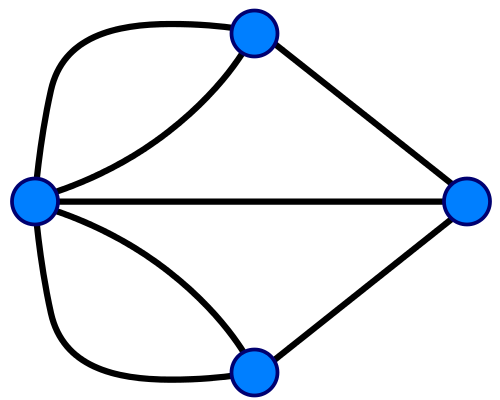
\includegraphics[width=0.3\linewidth]{Konigsberg_graph.png}
%	\caption[\selectlanguage{english}Konigsberg problem of seven bridges.]{The Kronigsber problem of seven bridges. The left panel shows the original map of the bridges; the right panel shows its graph representation. }

%	\label{fig:Krgraph}
%\end{figure}
%TODO review network models
The analysis of different real networks showed that they share common properties \cite{boccaletti2006complex}: small-world behaviour, large clustering and scale-free structure \cite{barabasi2009,newman2010}. Small-world property means that the distance between any two nodes is small and scales as logarithmic with the degree of the node. Real systems show high clustering, and the most prominent feature is scale-free property, where the degree distribution follows the power law. In the random network model (Erdős-Rényi) each node has an equal connecting probability, \cite{dorogovtsev2010complex}. This model produces Poisson degree distribution, contrary to those properties observed from data, so it could not describe real systems. Two seminal papers from 1999. by Watts and Strogatz \cite{watts1998collective}, and the Barabási-Albert model \cite{barabasi1999} inspired further research in this field. Watts and Strogatz  \cite{watts1998collective} proposed a new model that could generate networks with small-world properties, while the famous Barabasi-Albert model \cite{barabasi1999} finds the emergence of broad degree distribution to be a consequence of preferential attachment and network growth. 

%On the other hand, using topology to model complex systems has led to applicable, impactful insights in the social sciences. One example is the small world network,12 which emerges on a regular lattice topology when some links between a node and its local neighbors are reconnected to distant nodes. The rewiring creates short path lengths (connections betweenany two nodes) and high clustering coefficients (the links be-tween three neighboring nodes form triangles). Because socialscientists had independently discussed similar properties, theycould relate their theoretical foundations to an explicit gener-ative mechanism, the rewiring. \cite{schweitzer2018sociophysics}

Different complex networks models were proposed in order to better describe the dynamics of social and technological systems. As linking probability in the BA model is linear with node degree, one generalization was to introduce nonlinear dependence. Further, the linking probability may depend on the node age \cite{dorogovtsev2000b, dorogovtsev2001b}, or any other node property such fitness. Some models considered that nodes become inactive, or even that network grows through nonlinear number of links \cite{pham2016}. On the other hands were considered models with accelarated growth in the number of nodes \cite{sen2004}, in order to simulated exponential expansion of the online social systems. The empirical analysis of various online social systems show that their growth is time dependent and often accelerated \cite{liu2019}. The number of new nodes joining in time has trends and reflect the typical human behavior \cite{mitrovic2010a, mitrovic2012,mitrovic2015}. Uncovering the role of elementary processes in network evolution \cite{ghoshal2013uncovering}. The complex network models contribute to our knowledge about the connections between network topology and system dynamics and help us to understand the underlying mechanisms that lead to the emergence of the properties of the complex networks. % \cite{barabasi1999, tadic2001, mitrovic2009}. 

%Degree-degree anti-correlations of the Internet can be explained, at least to a certain extent, by single edge constrain \cite{maslov2004, park2003}. Detailed analysis of emergence of clustered networks shows that clustering is either the result of finite memory of the nodes \cite{klemm2002} or occurs due to triadic closure \cite{serrano2005}. 

%TODO: review sociophysics

The models have contributed to methods to explain the system's microscopic dynamics but also to computational approaches for modeling such systems \cite{schweitzer2018sociophysics}. These models have to inference with empirical data and social theories. Another example of succesful data-driven modeling is forecasting the spread of an epidemics. On the other hand it is also possible to model collective emotional dynamics, where hypothesis about emotional interactions are tested against data. \cite{garas2012emotional}. %ovo prepisati










%TODO: review social groups
%Social groups, informal or formal, are mesoscopic building elements of every socio-economic system that direct its emergence, evolution, and disappearance \cite{firth2013elements}. The examples span from countries, economies, and science to society. Settlements, villages, towns, and cities are formal and highly structured social groups of countries. Their organization and growth determine the functioning and sustainability of every society \cite{barthelemy2016structure}. Companies are the building blocks of an economic system, and their dynamics are essential indicators of the level of its development \cite{hidalgo2009building}. Scientific conferences, as scientific groups, enable fast dissemination of the latest results, exchange, and evaluation of ideas as well as a knowledge extension, and thus are an integral part of science \cite{smiljanic2016theoretical}. The membership of individuals in various social groups, online and offline, can be essential when it comes to the quality of their life \cite{montazeri2001anxiety, davison2000talks, cho2012tea}. Therefore, it is not surprising that the social group emergence and evolution are at the center of the attention of many researchers \cite{aral2012identifying,gonzalez2013broadcasters, torok2013opinions, yasseri2012dynamics}.\\


%The availability of large-scale and long-term data on various online social groups has enabled the detailed empirical study of their dynamics. The focus was mainly on the individual groups and how structural features of social interaction influence whether individuals will join the group \cite{backstrom2006group} and remain its active members \cite{smiljanic2016theoretical, smiljanic2017associative}. The study on LiveJournal \cite{backstrom2006group} groups has shown that decision of an individual to join a social group is greatly influenced by the number of her friends in the group and the structure of their interactions. The conference attendance of scientists is mainly influenced by their connections with other scientists and their sense of belonging \cite{smiljanic2016theoretical}. The sense of belonging of an individual in social groups is achieved through two main mechanisms \cite{smiljanic2017associative}: expanding the social circle at the beginning of joining the group and strengthening the existing connections in the later phase. Analysis of the evolution of large-scale social networks has shown that edge locality plays a critical role in the growth of social networks \cite{leskovec2008microscopic}. The dynamics of social groups depend on their size \cite{palla2007quantifying}. Small groups are more cohesive with continued long-term, while large groups change their active members constantly \cite{palla2007quantifying}.
%PNAS
%These findings help us understand the growth of a single group, the evolution of its social network, and the influence of the network structure on group growth. However, how the growth mechanisms influence the distribution of members of one social system among groups is yet to be understood.\\

%Furthermore, it is not clear whether the growth mechanisms of social groups are universal or system-specific. The size distribution of social groups has not been extensively studied. Rare empirical evidence of the size distribution of social groups indicates that it follows power-law behavior \cite{zheleva2009co}. 



%A related question that should be addressed is whether we can create a unique yet relatively simple microscopic model that reproduces the distribution of members between groups and explains the differences observed between social systems. French economist Gibrat proposed a simple growth model to produce companies' and cities' observed log-normal size distribution. However, the analysis of the growth rate of the companies \cite{amaral1997scaling} has shown that growth mechanisms are different from those assumed by Gibrat. In addition, the analysis of the growth of the online social networks showed that the population size and spatial factors do not determine population growth, and it deviates from Gibrat's law \cite{zhu2014online}. Other mechanisms, for instance, growth through diffusion, have been used to model and predict rapid group growth \cite{kairam2012life}. However, the growth mechanisms of various social groups and the source of the scaling observed in socio-economic systems remain hidden.\\



%%%%%%%%%%%%%%%%%%%%%%%%%%%%%%%%%%%%%%%%%%%%%%%%%%%%%%%%%%%%%%%%%%%%%%%%%%%%%%%%%%%%%


%The development of a knowledge-based society is one of the critical processes in the modern world \cite{leydesdorff2001sociological,leydesdorff2012triple}. In a knowledge-based society, knowledge is generated, shared, and made available to all members. It is a vital resource. Sharing this resource between individuals and organizations is a necessary process, and knowledge-sharing communities are one of the fundamental elements of a knowledge society.

%Often, these knowledge-sharing communities depend on the willingness of their members to engage in an exchange of information and knowledge. Participation in the community is voluntary, with no noticeable material gains for members. Thus, the exchange of knowledge depends on mutual trust between members. Trust that the community will consider their questions essential for the growth of the knowledge corpus and invest resources to answer their questions. Trust that the community will objectively evaluate their answers based on their quality and clarity. The trust mentioned is beyond the direct trust formed between two members. It is a feeling of a member that a community can be trusted and that their engagement is valuable. A feeling of community that a member can be trusted and expressed through engaging that member in community activities. It is a collective phenomenon that depends on and is built through social interactions between community members. This is why we believe it is crucial to understand how trustworthy knowledge-sharing communities emerge and disappear, as well as to unveil the fundamental mechanisms that underlie their evolution and determine their sustainability.

%In the past two decades, we have witnessed the emergence of an online knowledge-sharing community StackOverflow, which has become one of the most popular sites in the world and the primary knowledge resource for coding. The success of StackOverflow led to the emergence of similar communities on various topics and formed the StackExchange (SE) network.
%The advancement of Information and communication technologies (ICTs) have enabled faster and easier creation and sharing of knowledge, but also the access to a large amount of data that allowed a detailed study of their emergence and evolution \cite{dankulov2015dynamics}, as well as user roles \cite{saxena2021users}, and patterns of their activity \cite{santos2019activity, slag2015one, chhabra2020activity}. However, relatively little attention has been paid to the sustainability of SE communities. Most research focused on the activity and factors that influence the users' activity in these communities. Factors such as the need for experts and the quality of their contributions have been thoroughly investigated \cite{dev2018size}. It was shown that the growth of communities and mechanisms that drive it might depend on the topic around which the community was created \cite{santos2019self}. \\

%%%%%%%%%%%%%%%%%%%%%%%%%%%%%%%%%%%%%%%%%%%%%

%TODO: ovde o agent based modelima i dinamici na mrezama

The advances in understanding large complex networks have increased attention in analyzing the physical and dynamical processed on the top of them.  The spreading and diffusion phenomena raised questions about how viruses spread among network of people or even how blackout may spread. The robustness of these systems is often studied by percolation and spreading phenomena in complex networks. %ovo prepisati

The studies about the dynamics and structure of complex networks are necessary for understanding underlying mechanisms that shape complex systems. Real networks are much more heterogeneous than networks obtained in simple models. Links may be directed or undirected, they may have temporal dependencies, or we can simply deal with different types of interaction in one system. Different network representations deal with these specific features. %ovo prepisati

\selectlanguage{english}



\section{In this thesis}

In this thesis we use statistical physics and complex network approaches to model and empirically analyze online social systems. These systems consist of many users interacting in various ways on online platforms and could be represented by complex networks. In chapter \ref{Ch:Method}, we provide the methodology employed for this research. We describe the fundamental measures of complex networks and introduce basic complex network models. Section 2.5 reviews the most common probability distributions that characterize the properties of complex systems and outlines distributions fitting methods. Finally, we introduce the multifractality of the time-series and dynamical reputation model. 

The chapter \ref{Ch:signals} addresses the difference between network models where the growth in a number of nodes is constant and when it follows a non-trivial growth signal. This research aims to quantify how growth signals influence the structure of complex networks. Using the adapted ageing model \cite{hajra2004}, we use computer simulations to generate different kinds of complex networks. For more realistic real-world network simulations, growing signals are time series of new users from online social platforms, MySpace and Tech group from Meetup. They are described with trends, cycles and long-range correlations. Often time-series have multi fractal properties. The results of this study are published in \cite{vranic2021growth}, and they show the importance of growth signals in shaping the network structure because the scale-free networks, which represent real systems, are mainly altered. 

As research on social groups mainly focuses on a single group, there are remaining questions about the characteristics of the entire system. 
%It has been shown that the distribution of company sizes follows log-normal behaviour and remains stable over decades \cite{stanley1996scaling}, and similar results are found for the sizes of cities \cite{barthelemy2016structure, barthelemy2019statistical}. 
For example, the Tech group is only one of the groups around which Meetup users organize; many other groups are created worldwide so system constantly grow. 
%So far, there has been little research on the growth of online social groups. 
In chapter \ref{Ch:Groups} we will examine how groups on online social platforms grow. The results are summarized in the paper  \cite{vranic2022universal}. This research is based on the Reddit and Meetup data. From Meetup, we create two data sets, one with groups created in London and the other with groups created in New York, while for Reddit, we selected groups built before 2012. We are interested in explaining scaling behaviour in group size distribution and growth rates of group, identifying the growth mechanisms present in the system and providing the bipartite complex network model that can reproduce the universality found in the system.

Even though across complex systems we find the emergence of universal behaviour, for example, the scaling of the degree distribution of two groups is similar, different factors might influence its success. It is well known that many online groups may suddenly fall apart. These questions are the subject of the chapter \ref{Ch:Trust}, which main results are published in the paper \cite{vranic2022sustainability}. Here, we study the question-answer platform Stack Exchange; it has more than 200 different topic-specified sites where people help each other in answering questions. What is interesting about this system is that some sites were closed because they did not produce enough activity. For that reason, we selected the sites with the same topic that failed but later, when someone proposed the site again, it stayed active. We analyze the evolution of user interaction networks, here we use the temporal network approach and compare active and closed sites. We find that it is essential how the network users are distributed into a core-periphery structure \cite{gallagher2020clarified}. The core must selects firmly connected users, but their interaction with periphery has to be high. In other words, we need a trustworthy core to hold community. Introducing the Dynamical Reputation Model (DIBRM) \cite{melnikov2018toward}, based on user interaction sequences, we quantify how much users can be trusted and whether the community has a strong core. In the appendix \ref{App:SE} we briefly describe the Stack Exchange sites, in the appendix \ref{App:parameters} and \ref{App:sliding} discuss how we choose parameters  for DIBRM model while in appendix \ref{App:robust} we discuss the stability of inferred core-periphery structures. 

Finally, in the chapter \ref{Ch:Conclussion}, we draw the main findings of this thesis. 










